\chapter{Software design and development}
\label{ch:software}

Within this chapter, the software is described from a user's perspective and linked to the design implications provided in the \nameref{ch:analysis} and the \nameref{ch:frameworks} chapters. The software is implemented as a webapplication in order to facilitate easy access from any webbrowser with internet connectivity. For a more technical description of the server and client, the full server documentation is included within the Flashmap Server Documentation appendix on page~\pageref{app:documentation}, and the client source code within the \nameref{app:clientsource} appendix on page~\pageref{app:clientsource}. Finally, the complete source code is available on github\footnote{\url{https://github.com/mcvdenk/MasterThesis-Software}}.

\section{Page elements}

Each page is represented as a webpage containing 4 different page elements, which are the navigation menu, the instructions panel, the main viewer, and a button panel. Within the different views of the application, they generally preserve the same functionality and layout, and will be explained below after the description of the colour scheme.

\subsection{Navigation menu}

The navigation is centered at the top of the screen, displaying buttons for the pages of the applications and a button to contact the developer for help (see figure~\ref{fig:navmenu}).

\begin{figure}
    \centering
    
\includegraphics[width=.8\textwidth]{img/navmenu.png}
    \caption{The navigation menu}
    \label{fig:navmenu}
\end{figure}

\subsection{Instructions panel}

The instructions panel is the next element is placed below the navigation menu, and is reserved for providing the user with extra instructions where needed. It does not have a background colour, but it does have a fixed height in order to keep all elements at the same place independent of the length of the instruction.

\subsection{Main viewer}

The main viewer is the central element, and expands from the instruction panel to the button panel. Within this container, the main content of the specific view is displayed, such as the flashcard or concept map, the questionnaire, or the login form. In order to stand out from the rest of the page, it has a separate background with rounded corners. The background colour is somewhat lighter in comparison to the general background colour in order for the text to be better readable. The main viewer is also the container for visjs, which is a javascript library for rendering graphs in browsers.

\paragraph{Visjs} Since the content contained within the graph is dynamic because of the partial maps returned from the server, generated automatic layouts of graphs are necessary. Visjs is capable of two models for automatic layout, namely hierarchical and force-directed. As described in the \nameref{sec:cmapframework} section on page~\pageref{sec:cmapframework}, the initial idea was to render the graphs as hierarchical. Upon trying this with different subgraphs however it was found that automatic assignment for the different nodes on different hierarchical levels was not correctly done by visjs. This is mainly due to the two options for hierarchical layouts, namely hubcentered and directed. The idea of a hubcentered hierarchy is that the levels of the nodes within the hierarchy are based on the amount of other nodes directly or indirectly linked to this node. This works especially well for tree graphs, but a concept map is not a tree graph because of the cross-links. The other option, directed hierarchy, should make advantage of the directed edges by determining the levels of the nodes based on the direction of the edges. Unfortunately, this is implemented within visjs as only the root and the leaves being determined whether there are only incoming or outgoing edges, whereas the rest of the nodes are still placed based on the hubcentered layout, unlike in other graph layout engines such as DOT. 

Because this rendering leads to more confusing graphs, the force-directed layout was chosen instead, despite this resulting in a more cyclical graphs common in other visualisation techniques such as mind maps. This layout engine attempts to position the nodes in such a way that all edges are about equally long and there are as few crossing edges as possible. This is done by assigning forces among the set of edges and the set of nodes, for example for having all nodes an inverse gravity force and all edges a spring force.

The other settings in visjs include options for assigning colours fitting within the existing colour scheme, and for the user being able to reposition nodes if for example the edge labels are not readable because of overlapping with other edges.

\subsection{Button panel}

Finally, within the footer of the page, a button panel is included. Here the user can choose to for example show the correct answer to a flashcard, or confirm that he has read a certain section within the instructional material. The layout of this panel is exactly the same as that of the navigation menu.

\section{Learning process}
\label{sec:client_learning}

The core functionality of the client is reviewing the user instances. In general, every time an instance is reviewed, first the question or incomplete flashmap is prompted, the user thinks of the correct answer, the client shows the correct answer, and finally the user indicates whether his answer was correct or incorrect. Alternatively, the system can prompt whether the user has read a certain section from the textbook, indicate that the user is finished with learning for today, or state that there are no more instances left to review. Finally, the user can also undo his last submitted response. These use cases are elaborated below.

\subsection{Read source}

Every time the user is encountered with a flashcard or flashmap from a new section within the instructional material, the user is prompted whether this section has been read, since the rehearsal of items cannot be meaningful when the user is not familiar with the content. These prompts take often place at the beginning of a session so that the user does not have to interrupt a session. Furthermore, they prompt two sections ahead of the material currently being learned or reviewed by the user from the flashmap or flashcards in order to guarantee that the user is familiar with the material before learning the items. The user is prompted to read a section at most once per day. Within the main viewer the question "Did you read section 13.1 already? If no, read this now." is displayed in Dutch. The user can then press the "Read" button in the button panel, which will lead to prompting the first instance. This screen is simular for each subsequent section prompt.

\begin{figure}
    \centering
    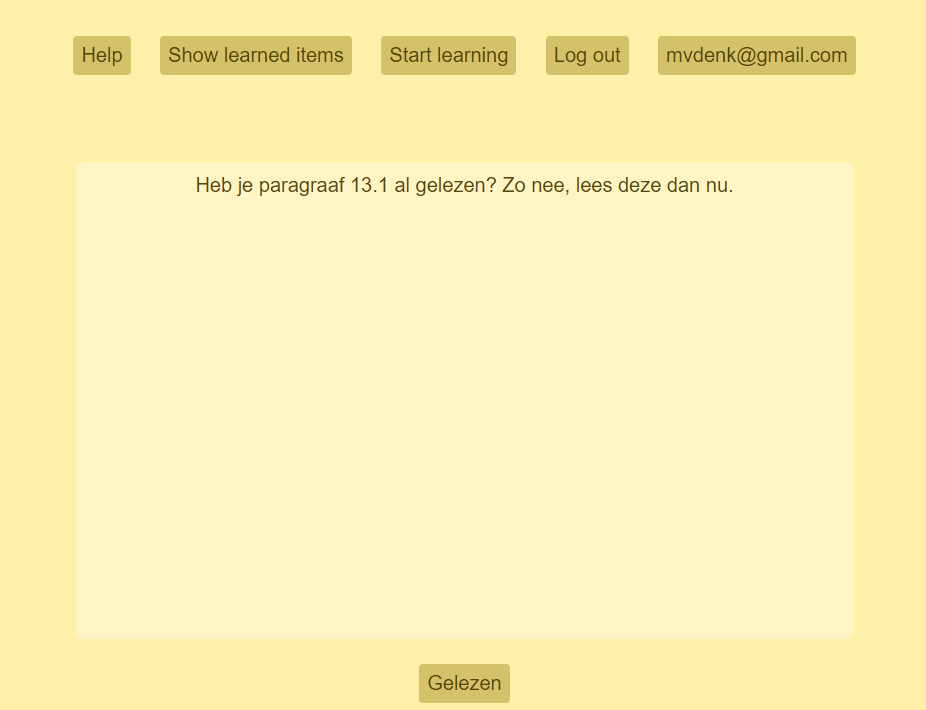
\includegraphics[width=.8\textwidth]{img/ui_read_request.png}
    \caption{The user interface when prompting the user whether he has read paragraph 13.1}
    \label{fig:ui_read_request}
\end{figure}

\subsection{Prompt}

When requesting items for review, the user can receive a due or new flashcard or flashmap, depending whether there are any old items due for review and the experimental group the user is in. If the user is a flashcard user, he will see the prompt such as in figure~\ref{fig:ui_fc_prompt}. The main viewer contains the specific flashcard question, and the button panel contains a button with the label "Show answer". The flashmap users get to see a partial incomplete flashmap within the main viewer (figure~\ref{fig:ui_fm_prompt}), which they can drag around and zoom in and out on. The cues which have to be retrieved are indicated by orange empty nodes.

\begin{figure}
    \centering
    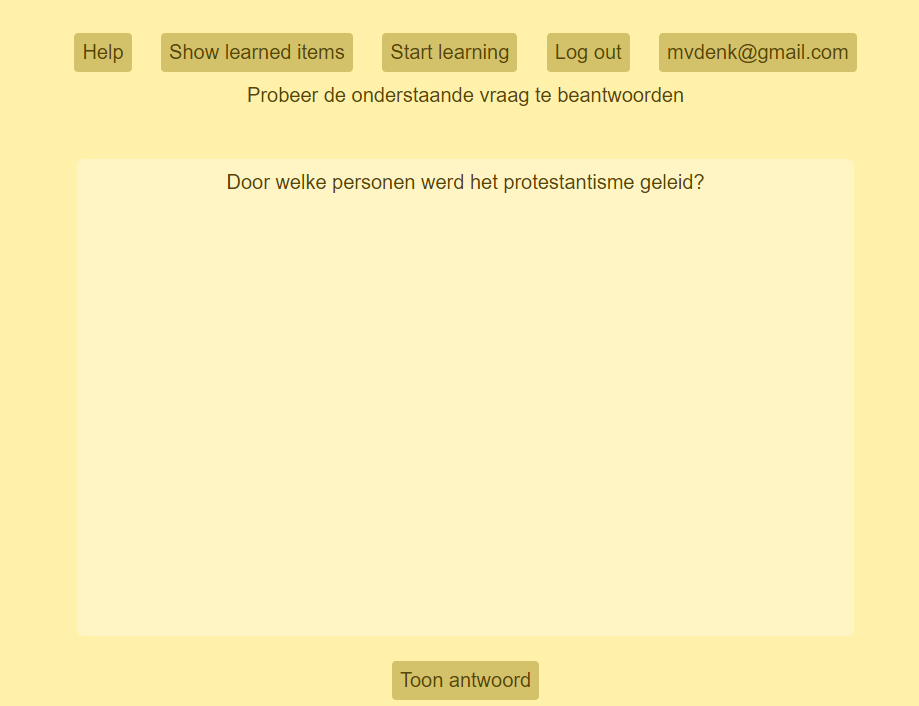
\includegraphics[width=.8\textwidth]{img/ui_fc_prompt.png}
    \caption{The user interface when prompting a flashcard}
    \label{fig:ui_fc_prompt}
\end{figure}

The partial map displayed to the user is a concept map containing all the concepts and relations which directly or indirectly point towards the relation which has to be learned (the parents), plus the concepts and relations linked to by the direct parent concept (the siblings). The reason why the parent concepts are returned rather than the child concepts is that in the instructional material the concepts are introduced top-down rather than bottom up, so building up the concept map from parent to child alligns better with the order in which the students read about the concepts. Additionally, the sibling nodes are also returned so that they can be prompted at the same time, and that the user has more context for deciding which concept should be filled in the missing node.

\begin{figure}
    \centering
    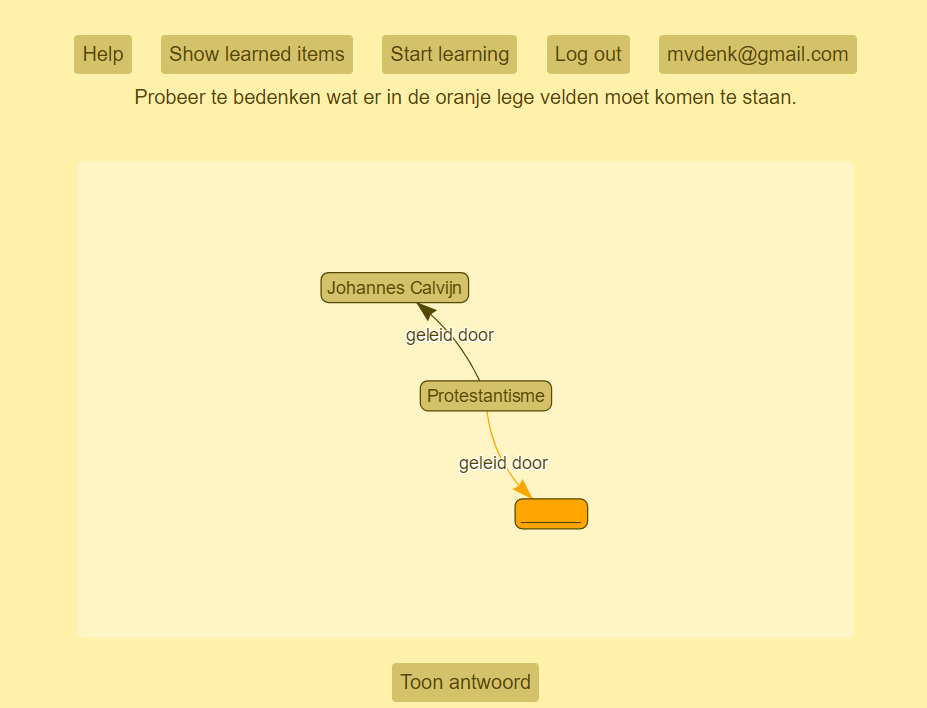
\includegraphics[width=.8\textwidth]{img/ui_fm_prompt.png}
    \caption{The user interface when prompting a flashmap}
    \label{fig:ui_fm_prompt}
\end{figure}

The button panel is the same for both conditions. The instructions element also shows instructions on what the user should achieve (to retrieve the correct answer from memory).

\subsection{Show answer}

After the user has pressed the "Show answer" button, the show answer prompt will be shown. Flashcard users get to see the correct answer in the main viewer below the question, with "Incorrect" and "Correct" buttons in the button panel to indicate whether the correct answer could be retrieved (figure~\ref{fig:ui_fc_answer}. Flashmap users get to see the correct answers within the previously empty nodes, which will also turn green indicating that the user retrieved them correctly (figure~\ref{fig:ui_fm_answer_correct}). When the user did not retrieve an answer correctly, he can click on that node, turning it red (figure~\ref{fig:ui_fm_answer_incorrect}). After the user indicated the correct and incorrect retrievals, he can click on a "Next" button in the button panel. The instructions element again contains instructions on what to do within this screen.

When the user has submitted at least one response within one session, he can undo this response if he is not content with it. For example, the user could after seeing the correct response decide that he thought of a similar enough answer, but after deeper reflection still decide that his answer was not sufficient. In this case, he could use the undo option in order to be presented with the previous response again and select the 'incorrect' option. The "Undo" button appears left to the "Show answer" button (see figure~\ref{fig:ui_undo}).

\begin{figure}
    \centering
    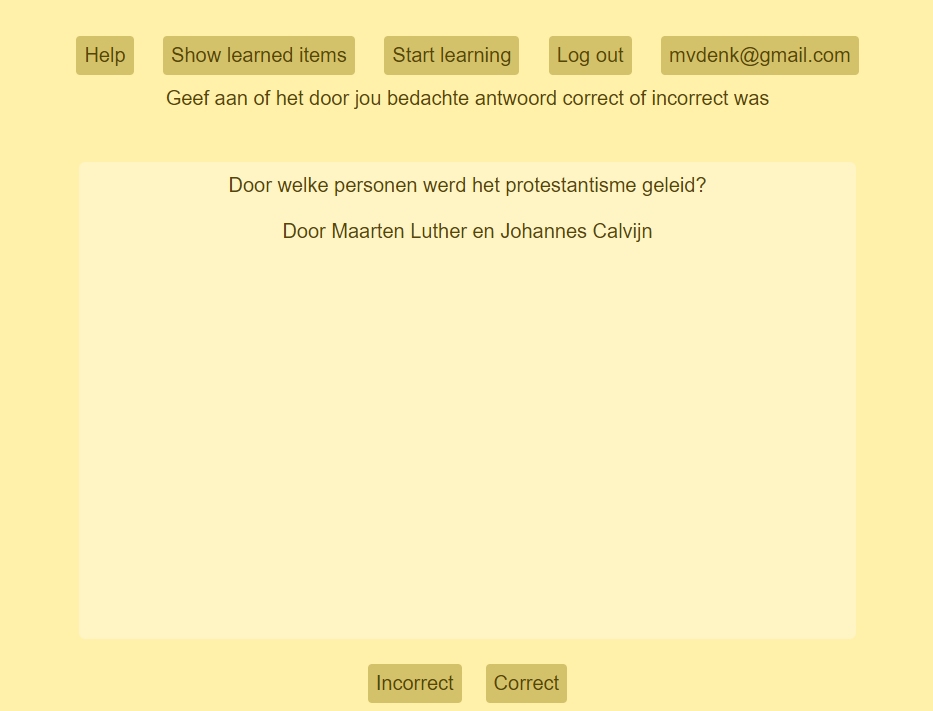
\includegraphics[width=.8\textwidth]{img/ui_fc_answer.png}
    \caption{The user interface when showing the answer to a flashcard}
    \label{fig:ui_fc_answer}
\end{figure}

\begin{figure}
    \centering
    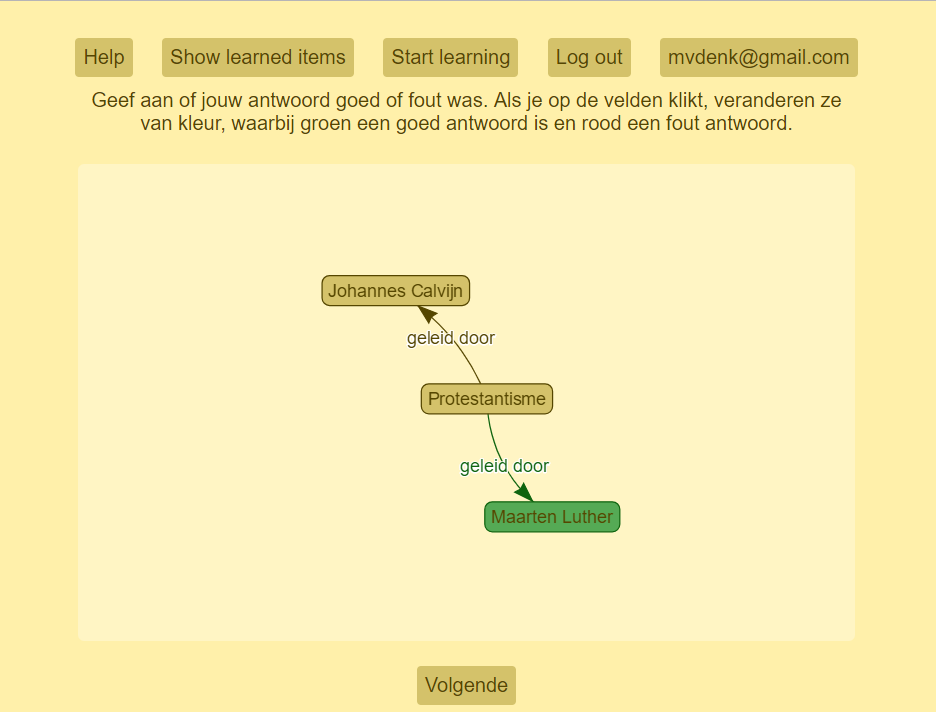
\includegraphics[width=.8\textwidth]{img/ui_fm_answer_correct.png}
    \caption{The user interface when showing the answer to a flashmap, here indicated as correct by the user}
    \label{fig:ui_fm_answer_correct}
\end{figure}

\begin{figure}
    \centering
    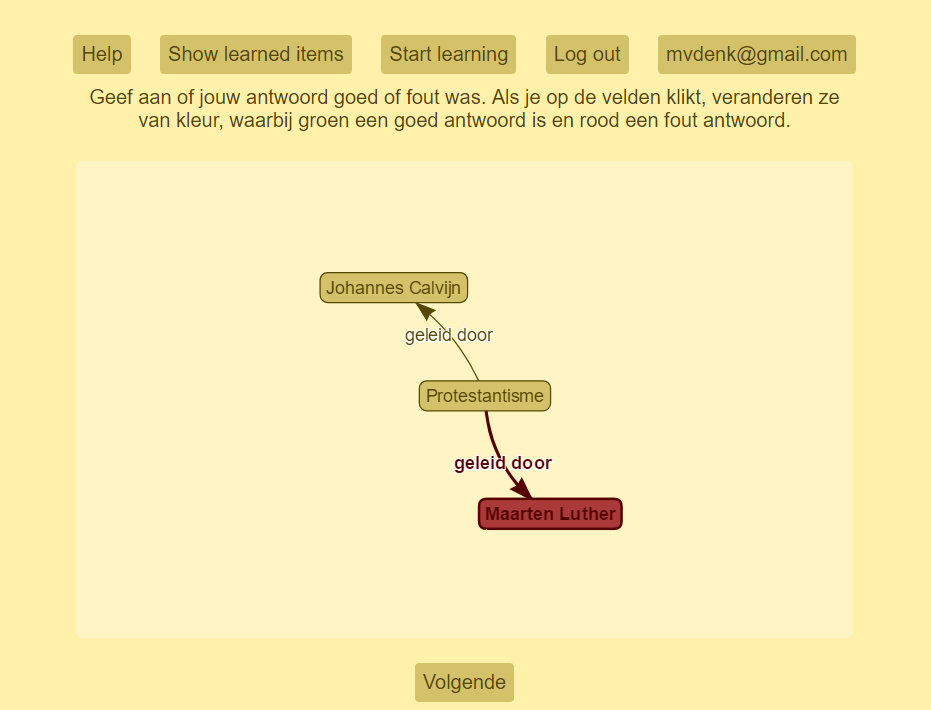
\includegraphics[width=.8\textwidth]{img/ui_fm_answer_incorrect.png}
    \caption{The user interface when showing the answer to a flashmap, here indicated as incorrect by the user}
    \label{fig:ui_fm_answer_incorrect}
\end{figure}

\begin{figure}
    \centering
    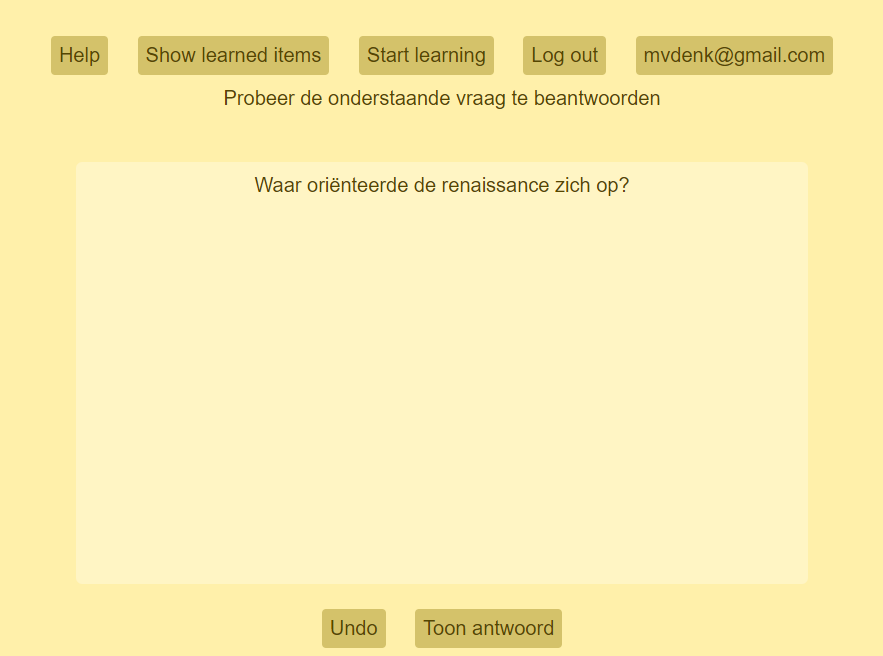
\includegraphics[width=.8\textwidth]{img/ui_undo.png}
    \caption{The user interface when prompting a flashcard with an undo option}
    \label{fig:ui_undo}
\end{figure}

After the user has provided the answer to the system, the system reschedules the flashmap or flashcard. In the~\nameref{subsec:adaptivesequencing} chapter on page~\pageref{subsec:adaptivesequencing}, it is described that in order to calculate the interval until the next review, one needs the number of correct responses since the last incorrect response. This is done by going through all the responses for the specific flashcard or flashmap in descending order of sent in date, increasing a counter until an incorrect response is found. Then, $5^{exp}$ seconds are taken as the interval until the next review of the flashcard or flashmap. Examples:
%
\begin{itemize}
    \item When there are no responses, the interval is $5^{1+0}=5$ seconds;
        \item When there are two correct responses, the interval is $5^{1+2}=125$ seconds;
        \item When there are two correct responses, followed by one incorrect response and then three correct responses, the interval is $5^{1+3}=625$ seconds.
\end{itemize}

\begin{figure}
\centering
    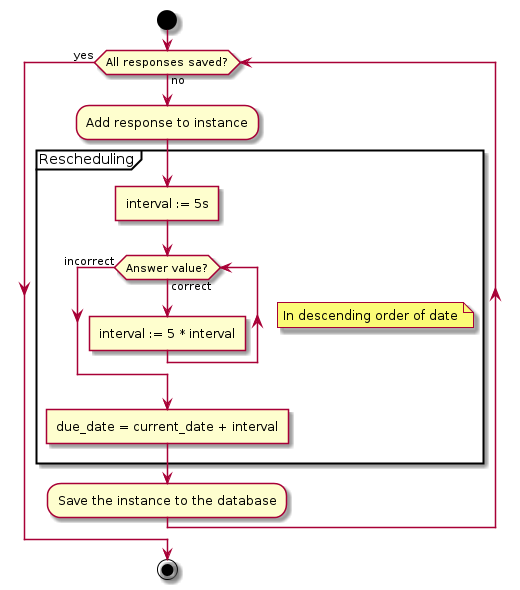
\includegraphics[height=.5\textheight]{img/learningserver.png}
\caption{An UML activity diagram showing the scheduling and saving of a list of responses within instances}
\label{fig:learningserver}
\end{figure}

\subsection{Finished learning and No more instances}

Finally, when the user has spent 15 minutes on the system or when there are no instances left to review, the user gets to see a screen such as in figure~\ref{fig:ui_no_more_instances}. The main viewer contains information on why the user is finished. When the user is finished because there are no more instances left in the sections he already read but there are still instances available in following sections, it also shows which section the user could read for the next instance, and presents a button to continue. Finally, if the user spent 6 days on the system, this prompt will also inform him that the next day he can take the posttest and fill in the questionnaire.

\begin{figure}
    \centering
    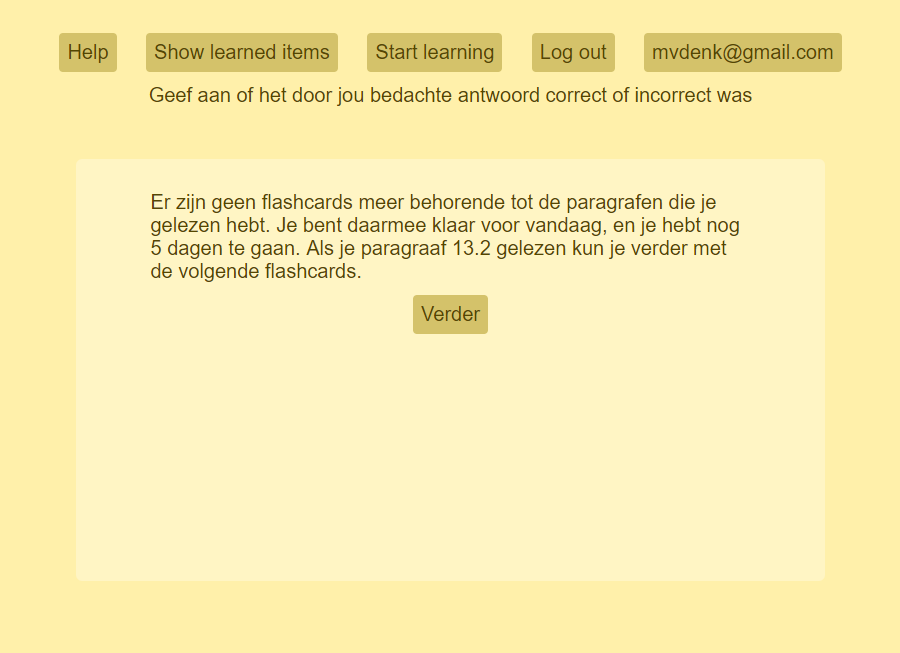
\includegraphics[width=.8\textwidth]{img/ui_no_more_instances.png}
    \caption{The user interface when showing that there are no new instances left to learn}
    \label{fig:ui_no_more_instances}
\end{figure}

\section{Other views}

Next to the main functionality described in the previous section there are also other views for accommodating the other use cases. For new users, these are the login screen, the descriptives screen, and the pretest, for regular users there are the help screen and the learning progress screen, and for the users which are finished there are the posttest, questionnaire, and debriefing screens.

\subsection{Login screen}

The main viewer in the login screen containing a simple form with a textfield for the username, and a submit button for logging in (figure~\ref{fig:ui_login}). Furthermore, a text within the instructions panel refers the users to the researcher's email adress for when they require further instructions or when the logging in does not function.

\begin{figure}
    \centering
    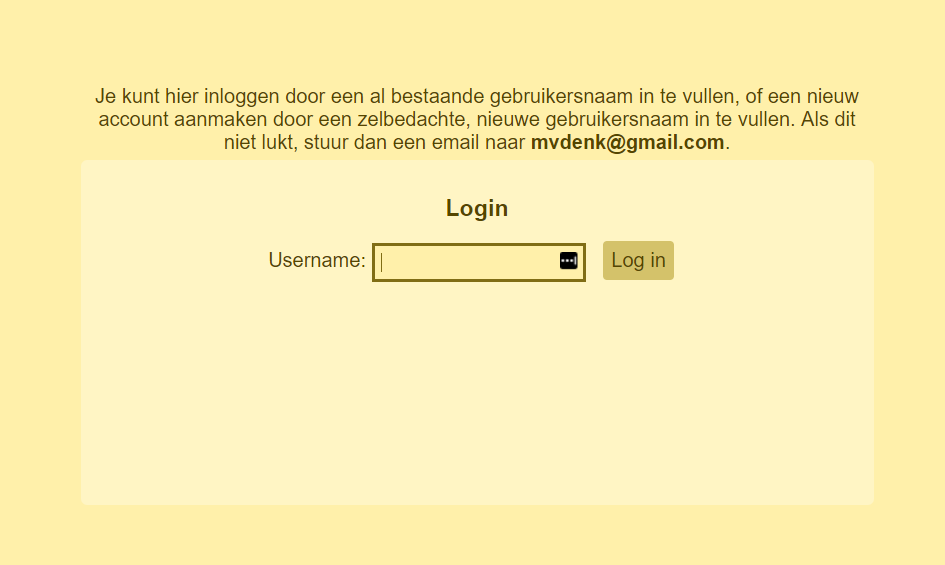
\includegraphics[width=.8\textwidth]{img/ui_login.png}
    \caption{The login screen}
    \label{fig:ui_login}
\end{figure}

\subsection{Descriptives, Test and Questionnaire forms}

These screens also contain basic forms, all containing questions or items and either textfields or radiobutton selection panels, depending on whether the question or item is open or closed, and a submit button at the bottom. (figures~\ref{fig:ui_descriptives}, \ref{fig:ui_test}, and~\ref{fig:ui_questionnaire}). The date field within the descriptives form is checked to be a valid date before the user can submit. Furthermore, the questionnaire item contains an email field for when the user wants to sign up for a later interview, which is a voluntary field and can be left empty. The instructions element again provide instructions for how to fill in the forms.

\begin{figure}
    \centering
    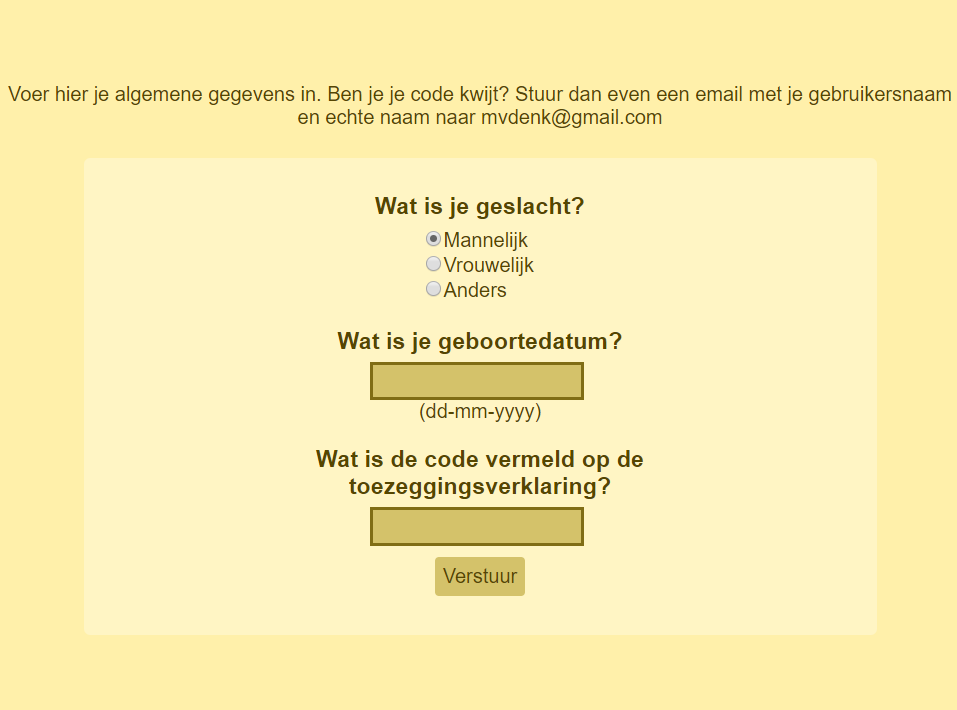
\includegraphics[width=.8\textwidth]{img/ui_descriptives.png}
    \caption{The descriptives screen}
    \label{fig:ui_descriptives}
\end{figure}

\begin{figure}
    \begin{subfigure}{0.4\textwidth}
        \centering
        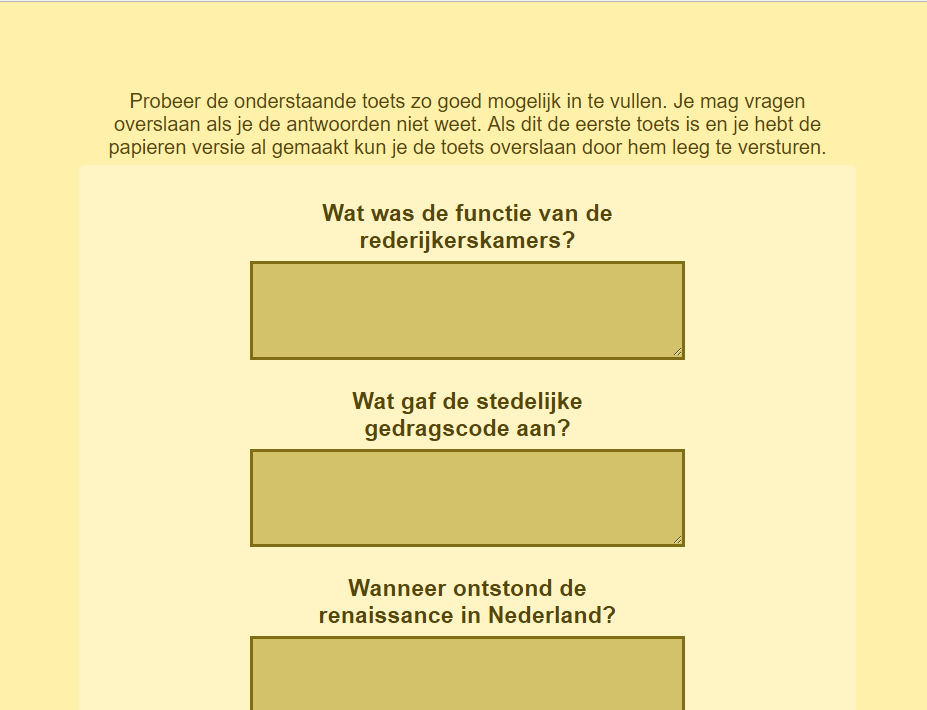
\includegraphics[width=\textwidth]{img/ui_test_top.png}
        \caption{Top}
        \label{fig:ui_test_top}
    \end{subfigure}
    \qquad
    \begin{subfigure}{0.4\textwidth}
        \centering
        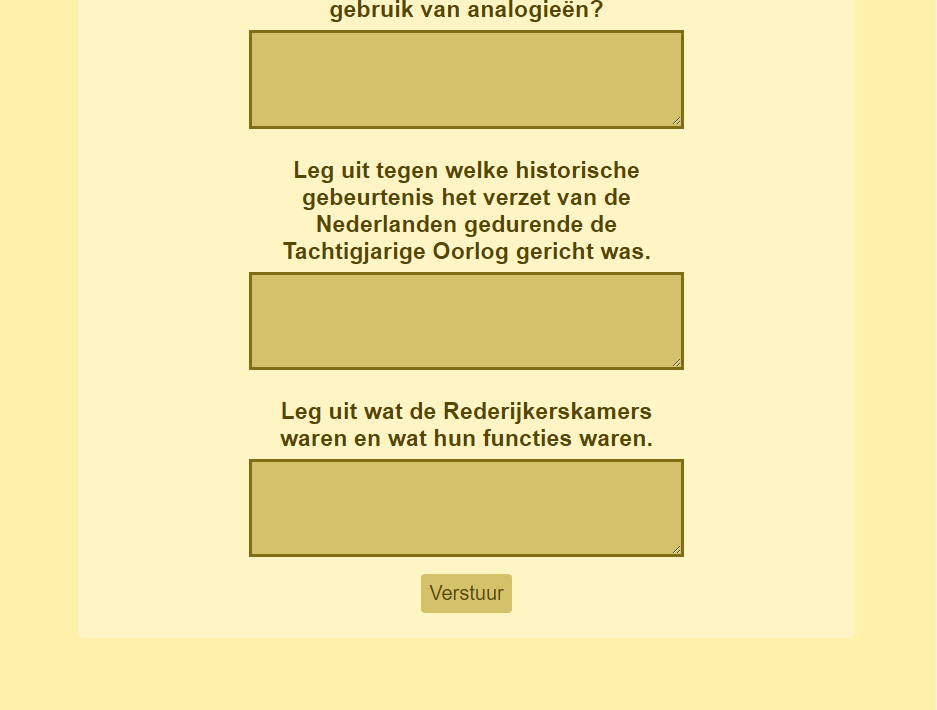
\includegraphics[width=\textwidth]{img/ui_test_bottom.png}
        \caption{Bottom}
        \label{fig:ui_test_bottom}
    \end{subfigure}
    \caption{The test screen}
    \label{fig:ui_test}
\end{figure}

\begin{figure}
    \begin{subfigure}{0.4\textwidth}
        \centering
        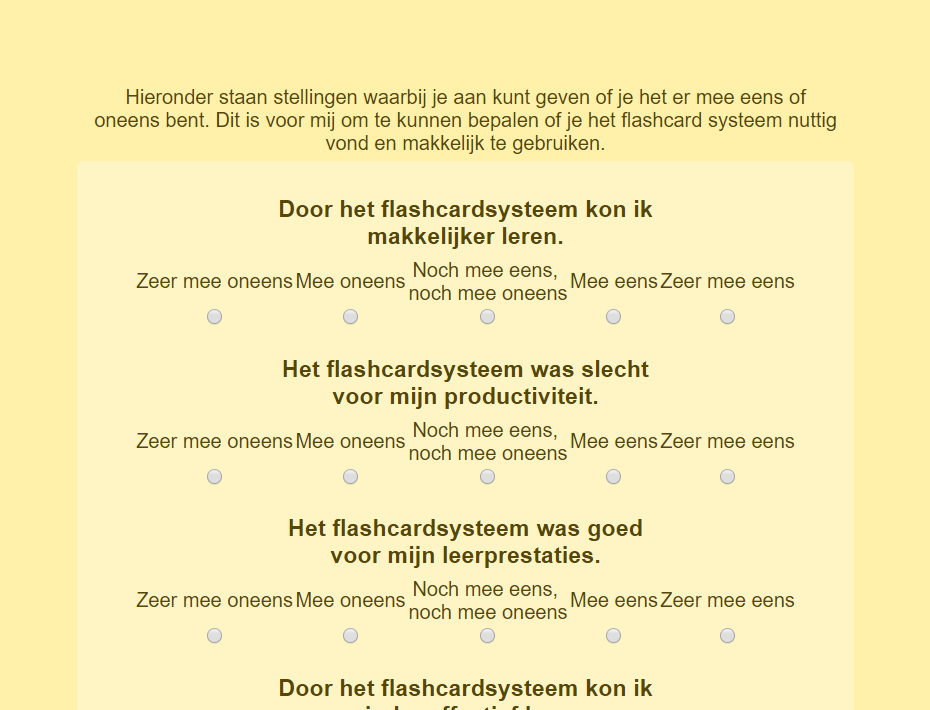
\includegraphics[width=\textwidth]{img/ui_questionnaire_top.png}
        \caption{Top}
        \label{fig:ui_questionnaire_top}
    \end{subfigure}
    \qquad
    \begin{subfigure}{0.4\textwidth}
        \centering
        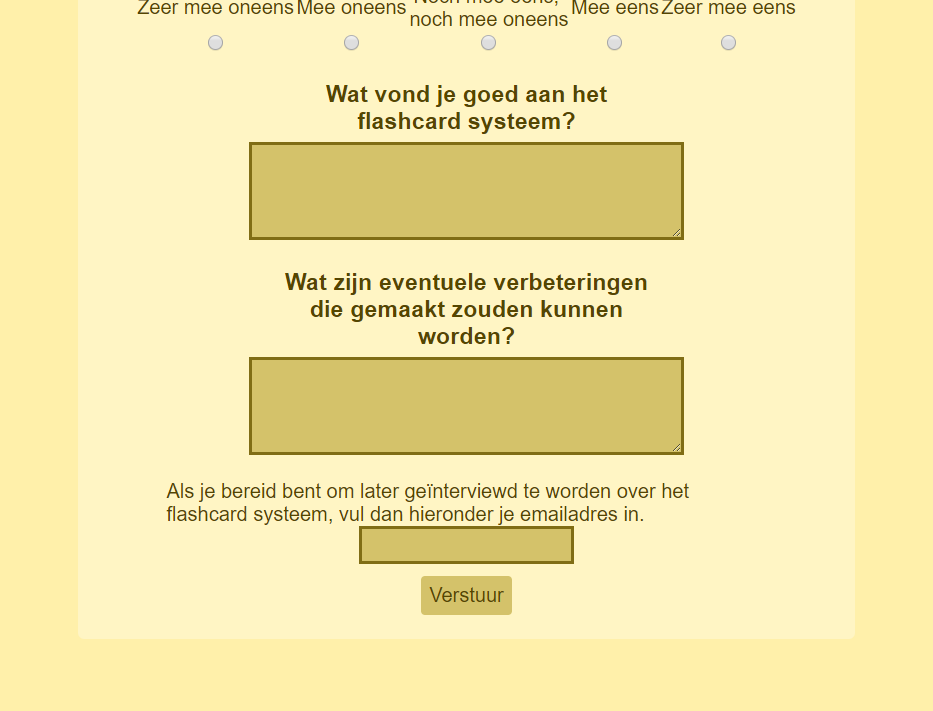
\includegraphics[width=\textwidth]{img/ui_questionnaire_bottom.png}
        \caption{Bottom}
        \label{fig:ui_questionnaire_bottom}
    \end{subfigure}
    \caption{The questionnaire screen}
    \label{fig:ui_questionnaire}
\end{figure}

\subsection{Debriefing}

Finally, when the user is finished using the system and filling in the posttest and questionnaire, the application presents the debriefing information (figure~\ref{fig:ui_debriefing}). This entails a thank you message, that the user will receive the coupon for ice cream soon, that he is able to keep using the system, that he can request his personal data gathered during the experiment from the researcher at any time, that he will receive an email for making an appointment for the interview when he filled in his email address, and that for further questions he can always send an email to the researcher's email address. When the user has read this information he can click the "Read" button.

\begin{figure}
    \centering
    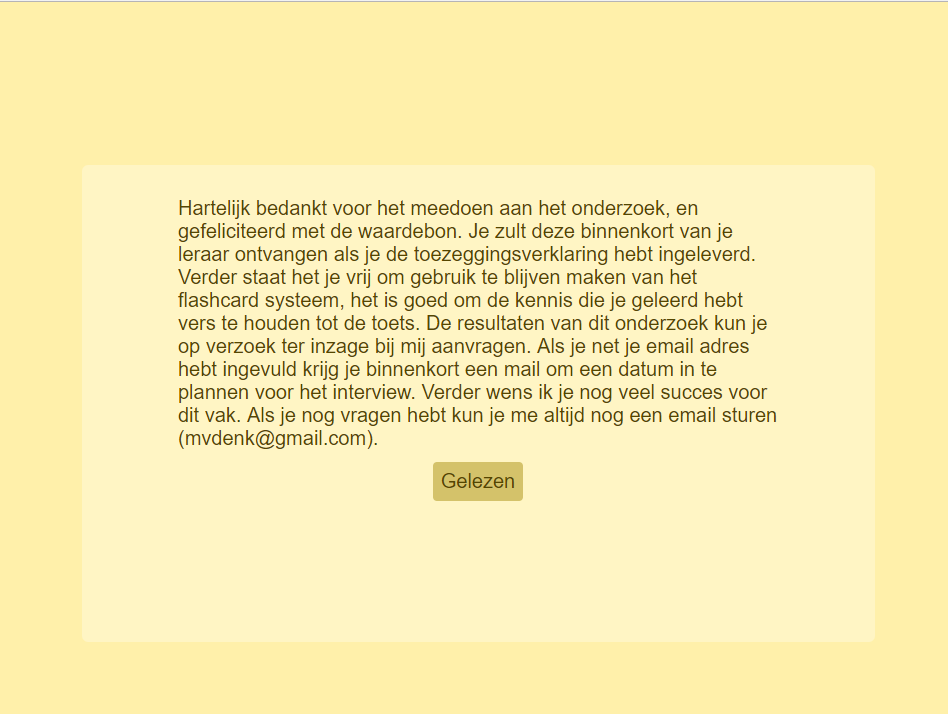
\includegraphics[width=.8\textwidth]{img/ui_debriefing.png}
    \caption{The debriefing screen}
    \label{fig:ui_debriefing}
\end{figure}

\subsection{Help}

The help screen (figure~\ref{fig:ui_help}) contains some global information about the experiment and on what conditions the user can receive the icecream coupon. It also states that the system will notify the user as soon as he is ready for today.

\begin{figure}
    \centering
    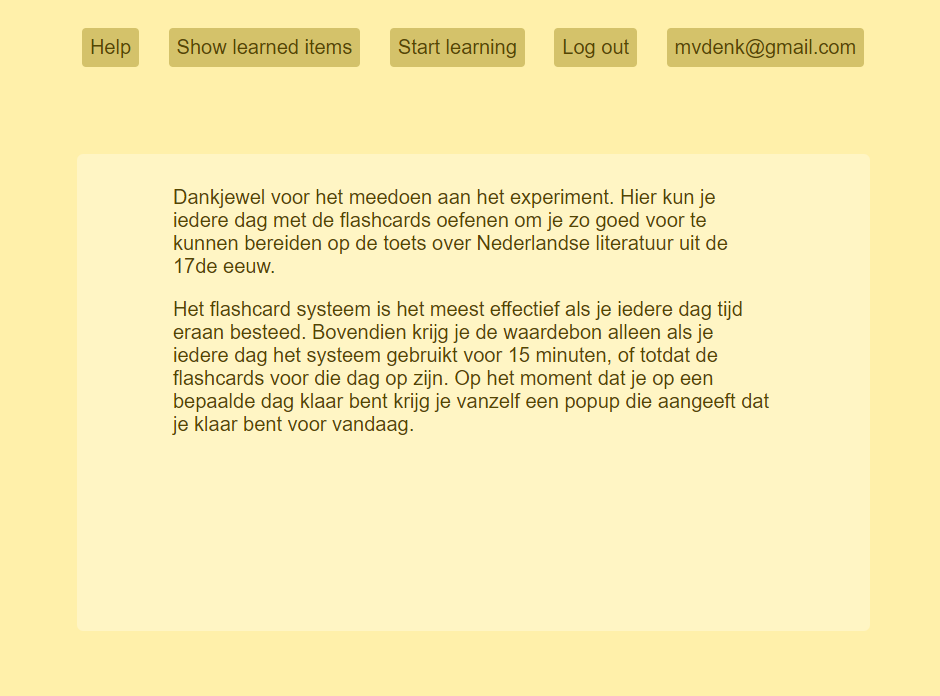
\includegraphics[width=.8\textwidth]{img/ui_help.png}
    \caption{The help screen}
    \label{fig:ui_help}
\end{figure}

\subsection{Learning progress}
\label{sec:learningprogress}

Finally, the user can request information about how much progress he made. Flashcard users are presented with how many cards are ready to be learned right now, how many are never reviewed, how many are new (less than exponent 2), how many are in the learning stage (less than exponent 6) and finally how many cards have been learned for the long term (more than exponent 6). Figure~\ref{fig:ui_fc_learnprogress_1} shows a learning progress screen of a new flashcard user, and figure~\ref{fig:ui_fc_learnprogress_2} an shows this overview for a user having correctly reviewed one flashcard but incorrectly reviewed another flashcard. The flashmap user is shown with a different overview, namely the part of the concept map containing the edges already reviewed by the user (figure~\ref{fig:ui_fm_learnprogress}), which will expand during the use of the system.

These views can still be improved in order to better convey the progress towards a user, which would contribute to a higher self-reinforcement. However, this has not yet been implemented due to time constraints.

\begin{figure}
    \begin{subfigure}{0.4\textwidth}
        \centering
        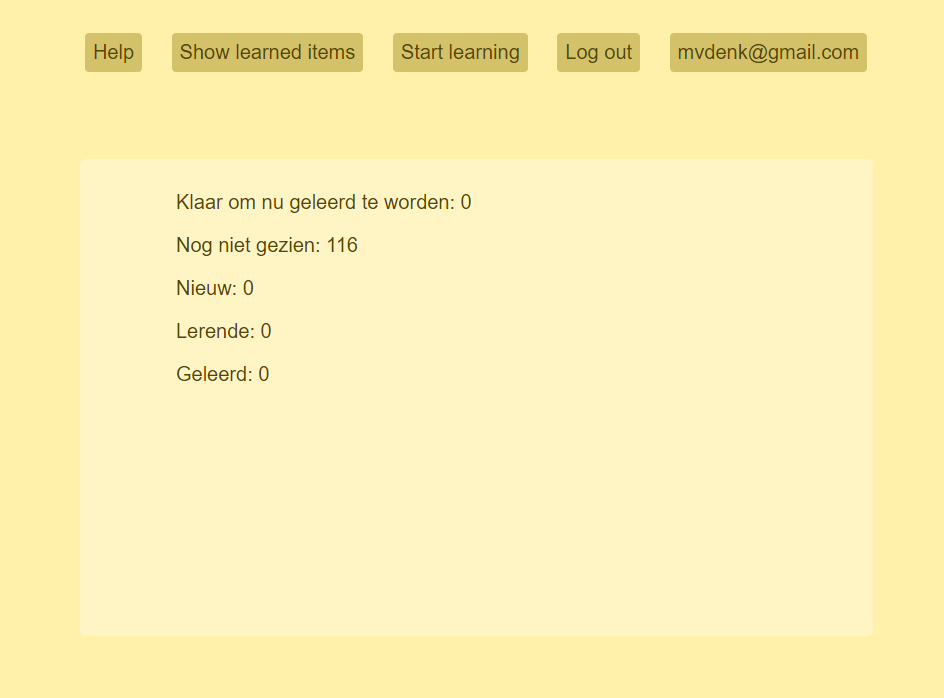
\includegraphics[width=.8\textwidth]{img/ui_fc_learnprogress_1.png}
        \caption{For a new flashcard user}
        \label{fig:ui_fc_learnprogress_1}
    \end{subfigure}
    \qquad
    \begin{subfigure}{0.4\textwidth}
        \centering
        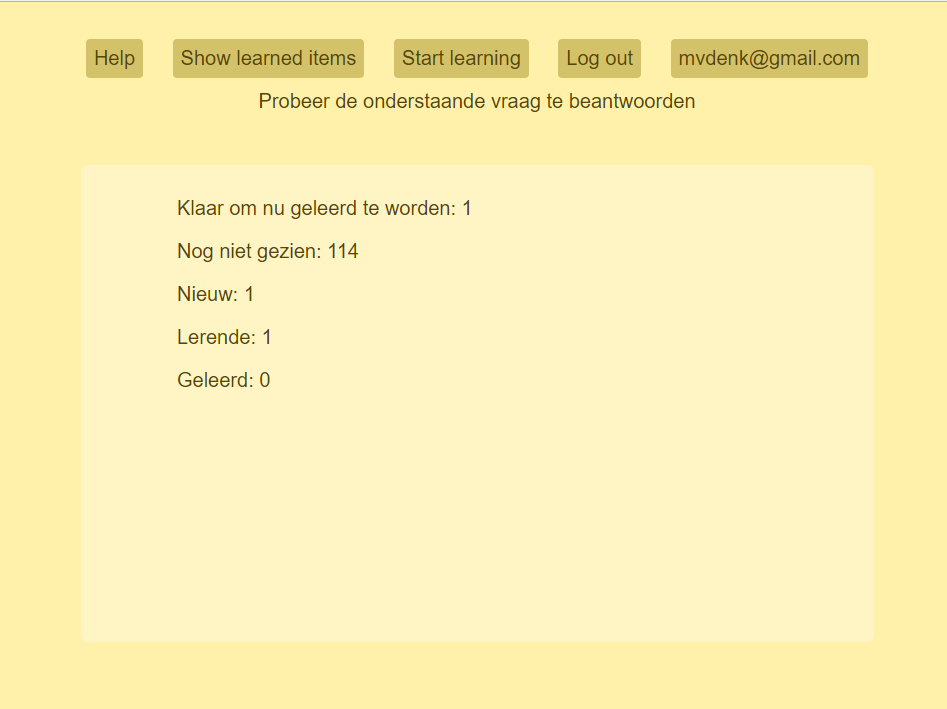
\includegraphics[width=.8\textwidth]{img/ui_fc_learnprogress_2.png}
        \caption{For a flashcard user having reviewed some flashcards}
        \label{fig:ui_fc_learnprogress_2}
    \end{subfigure}
    \caption{The user interface when showing the learning progress to a flashcard user}
    \label{fig:ui_fc_learnprogress}
\end{figure}

\begin{figure}
    \centering
    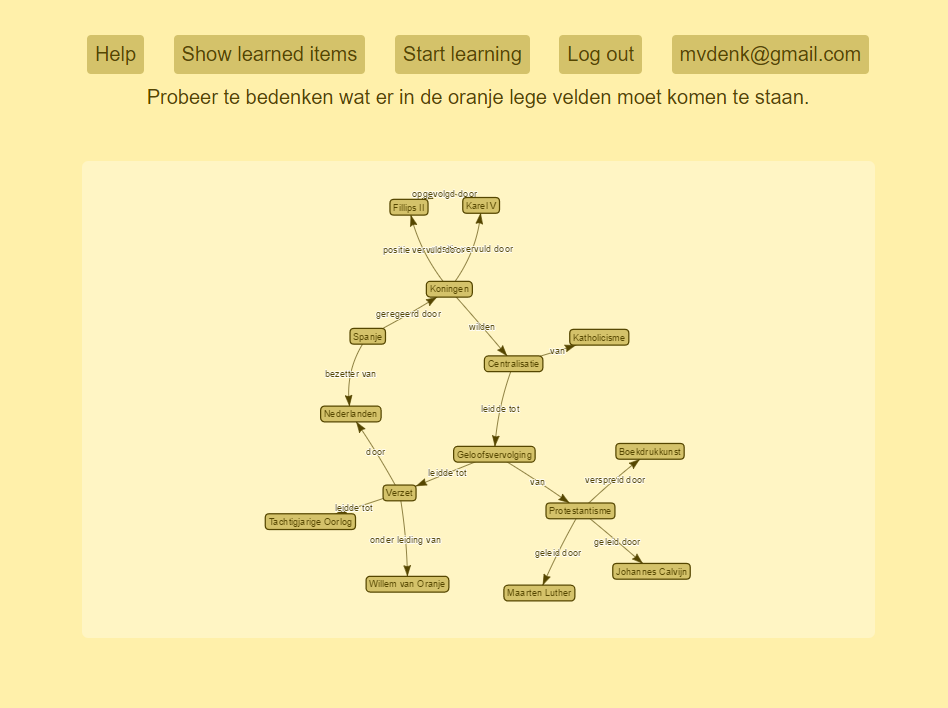
\includegraphics[width=.8\textwidth]{img/ui_fm_learnprogress.png}
    \caption{The user interface when showing the learning progress to a flashmap user}
    \label{fig:ui_fm_learnprogress}
\end{figure}

\section{Testing the software}

All of the above described functions are tested thoroughly using unittests (\url{https://github.com/mcvdenk/MasterThesis-Software/tree/master/server/unittest}) and using black-box tests from within the client.
